\documentclass[tikz,border=4pt]{standalone}
\usepackage{pgfplots}
\pgfplotsset{compat=1.18}
\begin{document}
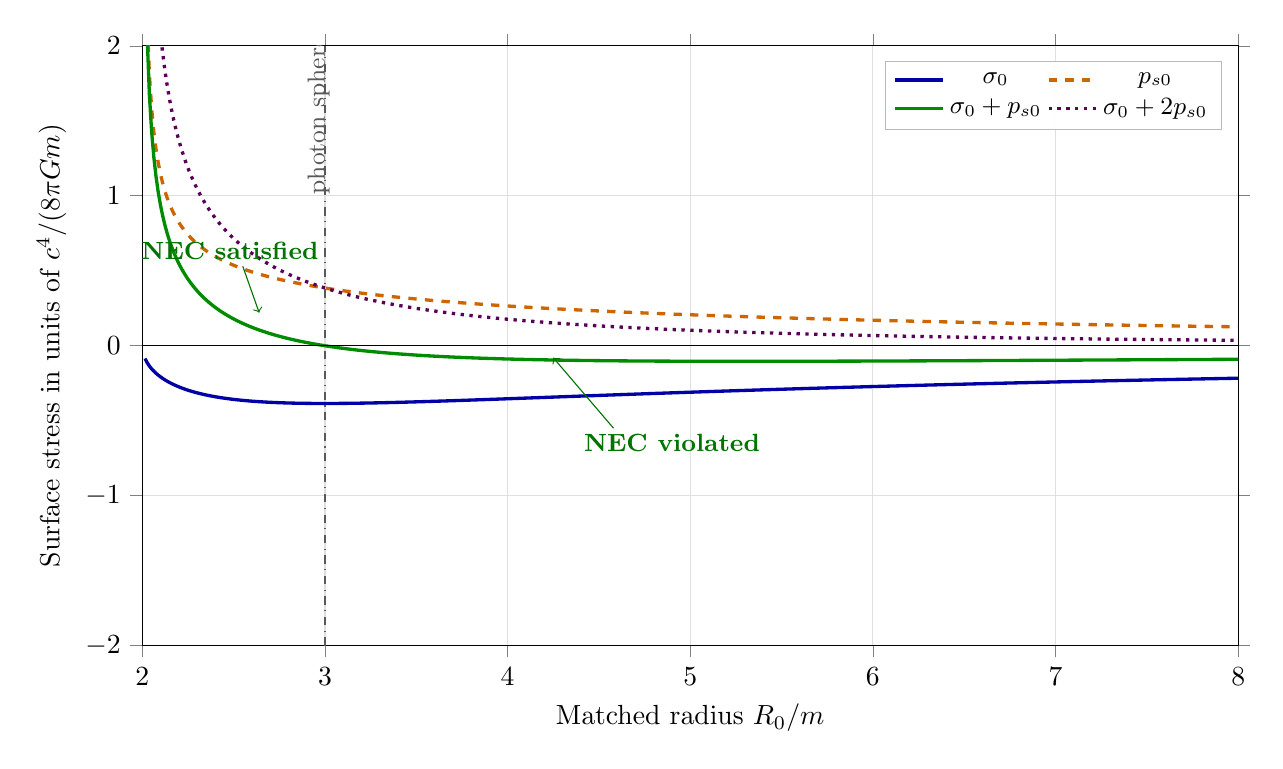
\begin{tikzpicture}
\begin{axis}[
  width=15.5cm,
  height=9.2cm,
  xmin=2,
  xmax=8,
  ymin=-2,
  ymax=2,
  xtick={2,3,4,5,6,7,8},
  ytick={-2,-1,0,1,2},
  xlabel={Matched radius $R_0/m$},
  ylabel={Surface stress in units of $c^4/(8\pi Gm)$},
  grid=major,
  grid style={gray!25},
  axis line style={black},
  tick align=outside,
  legend style={
    at={(0.985,0.975)},
    anchor=north east,
    draw=gray!55,
    fill=white,
    fill opacity=0.96,
    text opacity=1,
    legend columns=2,
    font=\small
  },
  samples=500,
  domain=2.015:8,
  clip=true
]
\addplot[blue!65!black,very thick] {-2*sqrt(1-2/x)/x};
\addlegendentry{$\sigma_0$}
\addplot[orange!80!black,very thick,dashed] {(x-1)/(x^2*sqrt(1-2/x))};
\addlegendentry{$p_{s0}$}
\addplot[green!55!black,very thick] {(3-x)/(x^2*sqrt(1-2/x))};
\addlegendentry{$\sigma_0+p_{s0}$}
\addplot[violet!70!black,very thick,dotted] {2/(x^2*sqrt(1-2/x))};
\addlegendentry{$\sigma_0+2p_{s0}$}
\addplot[black,thin] coordinates {(2,0) (8,0)};
\addplot[gray!70!black,dash dot,thick] coordinates {(3,-2) (3,2)};
\node[rotate=90,anchor=south,font=\small,text=gray!70!black]
  at (axis cs:3.08,1.9) {photon sphere $R_0=3m$};
\node[font=\small\bfseries,text=green!45!black] at (axis cs:2.48,0.63) {NEC satisfied};
\draw[->,green!45!black] (axis cs:2.55,0.53) -- (axis cs:2.64,0.22);
\node[font=\small\bfseries,text=green!45!black] at (axis cs:4.9,-0.65) {NEC violated};
\draw[->,green!45!black] (axis cs:4.58,-0.55) -- (axis cs:4.25,-0.08);
\end{axis}
\end{tikzpicture}
\end{document}
